\chapter{Concepts \& Design}\label{chapter::app-concepts-design}

\section{Introduction}
	An Application software or \textit{app} is a computer program designed to perform a specific set of tasks or actions for the end user. There are countless number of applications in use today and the majority of them are web applications following a centralized client-server model\cite{raval2016decentralized}.
	
	\begin{figure}[h]
		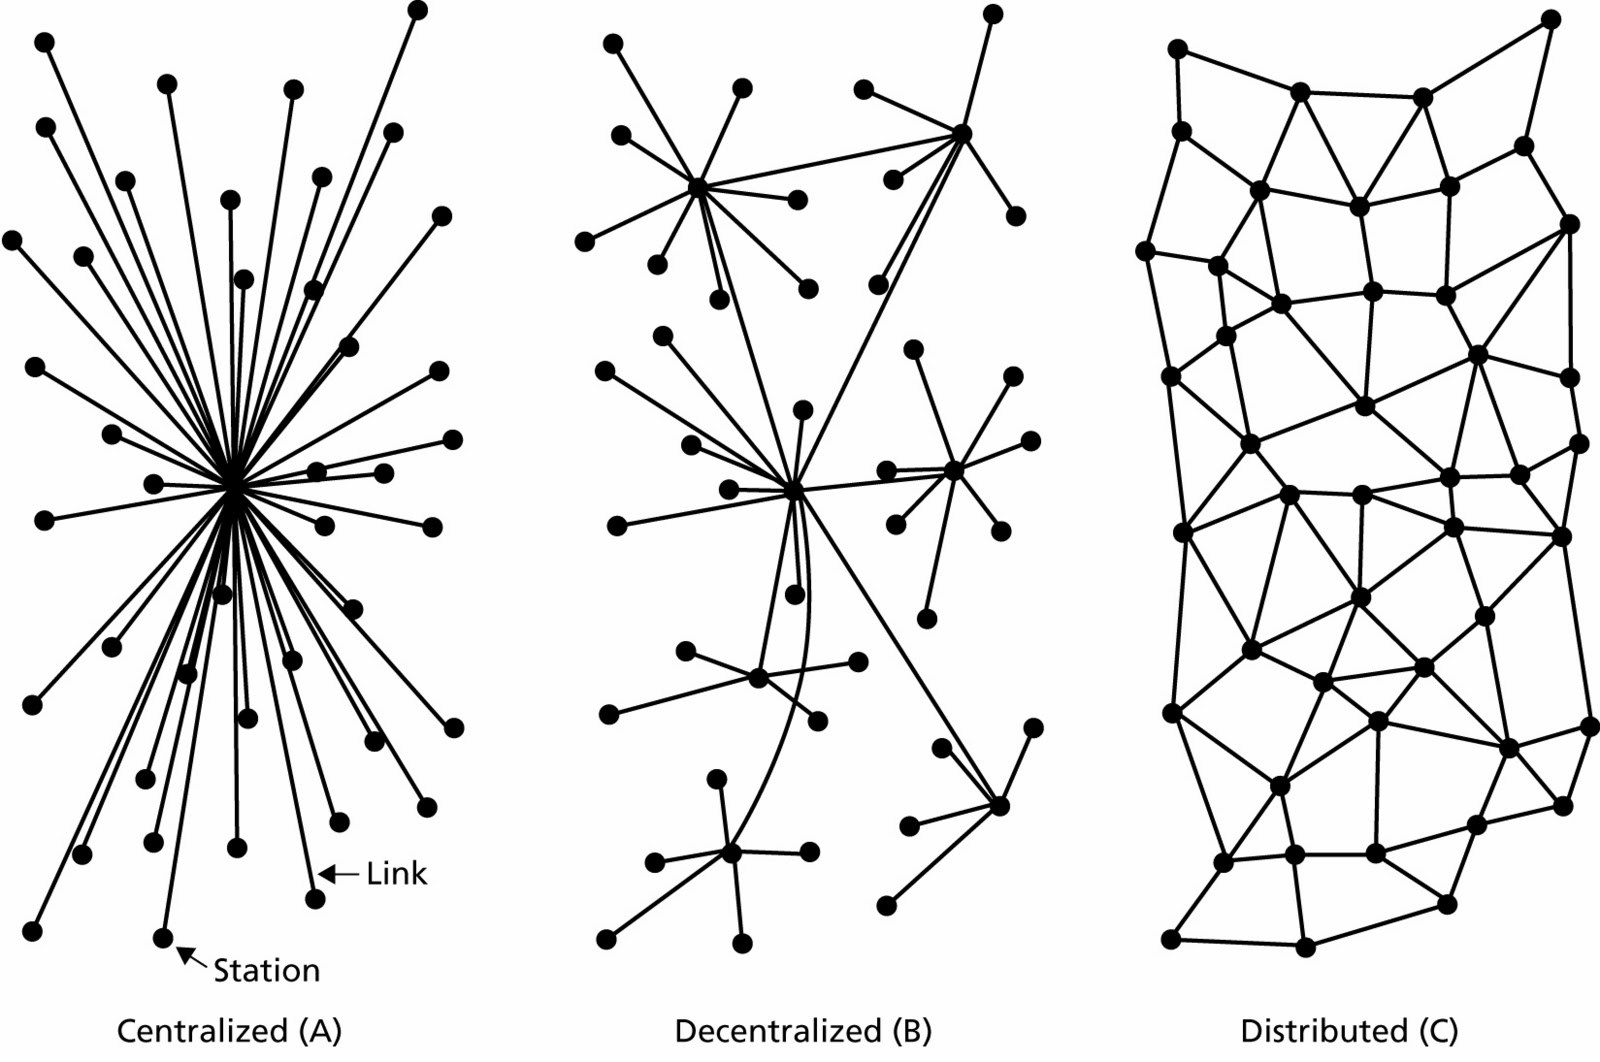
\includegraphics[width=\linewidth]{figures/network-models}
		\caption{\label{fig:applications} The three way of modeling web applications}
	\end{figure}
	
	Figure~\ref{fig:applications} shows a visual representation of three different ways of modeling web applications\cite{baran1964distributed}. Here, \textit{Centralized} and \textit{Decentralized} refers to level of control, while \textit{Distributed} refers to differences of location. Both centralized and decentralized systems can be distributed as well.
	
	\subsection{Centralized}
	It's currently the widespread way of building software applications. In this model a central server control the flow of information and governs the operation of individual units. Since the control is centralized, these types of systems suffer from single point of failure risk.
	
	\subsection{Distributed}
	In a Distributed model, the control still resides with a central server, however, the computation is spread across multiple nodes or servers.
	
	\subsection{Decentralized}
	In a Decentralized model, there is no central point of control as it's spread across all the servers running the application. Applications built using this model don't have a single point of failure and are inherently fault tolerant.

\section{Enabling Technologies}
	The document \textit{Information Management: A Proposal\cite{berners1989information}} written by \textit{Sir Tim Berners-Lee\footnote{\url{https://www.w3.org/People/Berners-Lee/}}} conceived the ideas for what would become the WorldWideWeb. It's main goal was to enable information exchange between computers in an accessible way at CERN\footnote{\url{https://home.cern/}}.
	
	HTML\footnote{\url{https://developer.mozilla.org/en-US/docs/Web/HTML}}, URI\footnote{\url{https://tools.ietf.org/html/rfc3986}} and HTTP\footnote{\url{https://tools.ietf.org/html/rfc2616}} were the fundamental technologies that defined the foundation of the Web. HTTP connected every computer on the planet with a common protocol. The HTTP protocol guidelines defined a set of trusted servers that translated a web address into a server address. Furthermore, HTTPS\footnote{\url{https://tools.ietf.org/html/rfc2818}} added another layer of trusted servers and certificate authorities. People would host personal servers for others to connect to, and everyone owned their data\cite{raval2016decentralized}. As the Web evolved, applications servers\footnote{\url{https://en.wikipedia.org/wiki/Application_server}} became the common way of interactive with the Web and the centralized model of data ownership as we know it today was born\cite{raval2016decentralized}. It was conceptually and programmatically easier to maintain an application server and profit from user's data that utilize it.
	
	Blockchain is the primary technology that enables the creation of applications with a decentralized model of data ownership. It puts the users of an application in control of their data thereby enabling a more open Web, as it was originally intended\footnote{\url{https://webfoundation.org/about/vision/history-of-the-web/}}.
	
	The blockchain helped solve the Byzantine Generals Problem\cite{lamport1982byzantine}. This problem describes a situation where all participating nodes in a distributed network must agree upon every message that is being transmitted between nodes, but where some of the nodes are corrupt and disseminating false information or are unreliable. This agreement is called as \textbf{consensus}. With Bitcoin\cite{nakamoto2008bitcoin}, decentralized consensus became possible. Agreement is achieved in the Bitcoin network by way of \textit{proof-of-work\footnote{\url{https://en.bitcoin.it/wiki/Proof_of_work}}} consensus mechanism which is resistant to Sybil Attack\cite{douceur2002sybil}. Proof-of work is both computationally and energy expensive; other consensus mechanism such as \textit{proof-of-stake\footnote{\url{https://en.bitcoin.it/wiki/Proof_of_Stake}}} relies on stake in the system instead of computational power.
	
\section{Application Concepts}
	There are five concepts in a web application that have traditionally been implemented in way that puts control with a centralized entity: data, identity, value, computing and bandwidth\cite{raval2016decentralized}. Each of these require trust in a 3rd party - a trust which can be betrayed. Recent advancements in distributed-system technology can put users in control of these things. Below sections describes each concept in detail and shows how one can build applications in a way such that centralized control is not required.

\section{Data}
	Data is the most important concept in any web application. First, let's look at how traditional web applications interact with data. Whenever, a user logs into an application, the application connects to a remote server and sends the authentication details. These details lets the server know which user is interacting with the application. Once authenticated, the user data is fetched from the remote storage and displayed to the user. All complex computations and data storage occurs on dedicated servers maintained in the cloud.
		
	\begin{figure}[h]
		\centering
		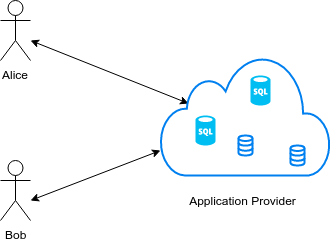
\includegraphics[width=200pt, height=150pt]{figures/traditional-app}
		\caption{\label{fig:traditional-app} How traditional web applications work}
	\end{figure}
		
	Figure~\ref{fig:traditional-app} shows how users interact with a traditional web application. Whenever, Alice wants to interact with Bob, she sends a message to the application server which then delivers the message to Bob. There is no direct path between Alice and Bob. This results in centralization where the provider acts as an intermediary between Alice and Bob's interaction; effectively governing how data is stored and shared among them.
		
	This model of application interaction requires that we trust the providers with out data and hope that they won't misuse or sell our data without our permission. Since revelations by Edward Snowden\cite{greenwald2014no}, we now know that trust can, has and will be broken as long as we entrust our data to a central entity\cite{raval2016decentralized}. Centralized stores of data also serve as a tool for surveillance, allowing big entities to monitor our internet behaviour without our knowledge. Cloud providers, despite having a distributed backend, are centrally owned.
		
	Additionally, as we move from a labor-based economy to an information-based economy, data will become the primary form of value. Therefore, its important that we not only possess our data, but own it as the world evolves. An ideal solution that enables this should provide a way of storing data in a decentralized way that is robust and as trustless as possible\cite{raval2016decentralized}.
	
	\subsection{Storing Data Directly in a Blockchain}
		This method does solves the decentralization of data as everyone who has copy of the Blockchain is storing the data but cannot alter it. The data can be encrypted such that it can only be accessed by someone having the private key. However, Blockchains were not meant for storing large amounts of data. It was designed for storing simple transactional logs, as its evident from looking at the Bitcoin Blockchain where individual records are in bytes\footnote{\url{https://en.bitcoin.it/wiki/Transaction}} and therefore cannot hold much data. Moreover, the Blockchain architecture implies that each node in the network must store a complete copy of the Blockchain. Therefore, storing a significant amount of data on a Blockchain is both expensive and impractical.
		
	\subsection{Storing Data in a Distributed Hash Table}
		DHTs ensure data resiliency by enabling easy distribution and indexing of data. Early peer-to-peer (P2P) filesharing applications like KaZaA\cite{good2003usability}, Napster\cite{ku2002creative} and Gnutella\cite{ripeanu2002mapping} used their own versions of DHTs with a varying degree of decentralization. Some had centralized trackers to monitor the movement of data, while some had central sources from which all data must pass, leaving them with single point of failure\cite{raval2016decentralized}.
		
		BitTorrent\cite{cohen2008bittorrent} was the first protocol to popularize DHT for sharing of large files. As of 2013, BitTorrent has 15–27 million concurrent users at any given time\cite{wang2013measuring}. The BitTorrent Mainline DHT serves as a decentralized data store with centralized trackers to monitor the network. It uses a tit-for-tat strategy between seeders and leechers to maximize the bandwidth of data distribution. This makes the BitTorrent protocol the de facto method for transfer of large datasets over the web. However, using BitTorrent as a data store is not feasible as there is no incentives for nodes to store a data leading to \textit{data impermanence}.
		
		Along with the decentralized storage capabilities of DHT and the speed of BitTorrent's protocol, we also want data permanence. Therefore, its necessary to incentivize the nodes storing the data in some way. Moreover, we also need to ensure that the links to the data don't die, an idea which was first proposed in Project Xanadu\cite{rayward1994visions}.
		
		\subsubsection{InterPlanetary File System (IPFS)}\label{sec:ipfs}
			IPFS\cite{benet2014ipfs} is a peer-to-peer file transfer protocol that implements these features, enabling a more permanent, decentralized Web, where links don't die and no single entity controls the data. It achieves this by combining previous peer-to-peer technologies such as DHT, BitTorrent and Git\cite{loeliger2012version}. Data in the IPFS network is modeled as a \textit{merkleDAG\footnote{Similar to a Merkle tree data structure, however, they do not need to be balanced and it's non-leaf nodes can contain some data.}}, a simple data structure that can be conceptualized as a series of nodes connected to each other\cite{raval2016decentralized}. This makes IPFS a \textit{content-addressed\footnote{A content-addressed storage is way to store information such that it can retrieved based on its content and not its location.}} system allowing efficient data lookup and retrieval as it doesn't rely on a single server to access the data.
		
			\begin{figure}[h]
				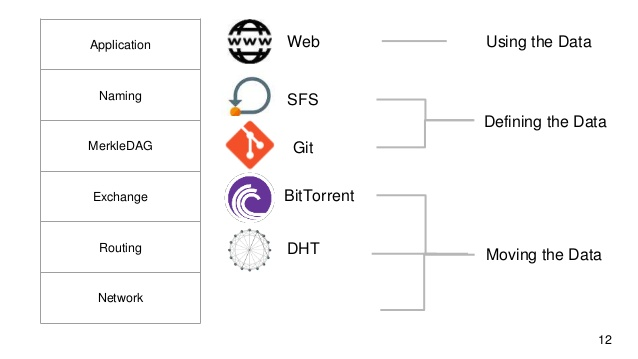
\includegraphics[width=\linewidth]{figures/ipfs-stack}
				\caption{\label{fig:ipfs-stack} IPFS Stack}
			\end{figure}
		
			Filecoin\cite{benet2018filecoin}, a \textit{decentralized storage network}, combines IPFS (shown in Figure~\ref{fig:ipfs-stack}\footnote{Adopted from: \url{https://image.slidesharecdn.com/ipfs-171229085327/95/ipfs-12-638.jpg?cb=1514537643}}) with an incentive structure that turns cloud storage into an algorithmic market effectively overcoming the limitations of BitTorrent. This market runs on a blockchain with a native protocol token, which miners earn by providing storage to clients.
		
	\subsection{Storing Data in a Cloud in Encrypted Containers}
		IPFS enables a way for decentralized storage such that it overcomes the single point of failure risk, however, the user does not control where the data is being stored. Because of this, once a data is added to the network, and is picked up by other nodes for re-hosting, it cannot be taken back as there is no way to verify information deletion\footnote{\url{https://github.com/ipfs/faq/issues/9}}.
		
		\subsubsection{Gaia: User-Controlled Storage}\label{sec:blockstack-gaia}
		Gaia\cite{ali2016blockstack} is a decentralized storage system that enables user-controlled private data lockers. It works by hosting data in one or more existing storage systems of user's choice. Data on Gaia is encrypted and signed by user-controlled cryptographic keys before being uploaded to a provider. Storing data using existing cloud infrastructure ensures high data availability without compromising on application performance. Further, since each data is signed by keys which a user controls, it ensures that they don't need to trust the underlying cloud providers.
		
		\begin{figure}[h]
			\centering
			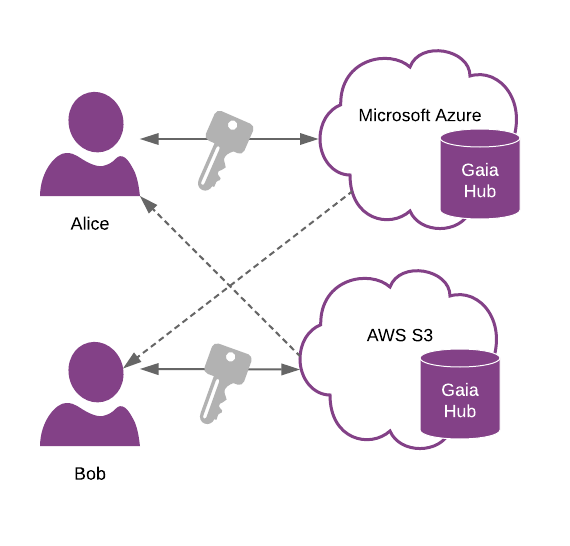
\includegraphics[width=200pt, height=200pt]{figures/gaia-storage}
			\caption{\label{fig:gaia-storage} How users interact with Gaia storage\protect\footnotemark}
		\end{figure}
		\footnotetext{\url{https://docs.blockstack.org/storage/overview.html}}
		
		Writing data to a Gaia hub involves a \texttt{POST} request along with a signed \textit{authentication} token. This token is signed by the private key which controls the particular bucket being written to. Separate buckets are used for each application, this ensures that a given private key grants access only to a specific bucket on the Gaia Server.
		
		\begin{figure}[h]
			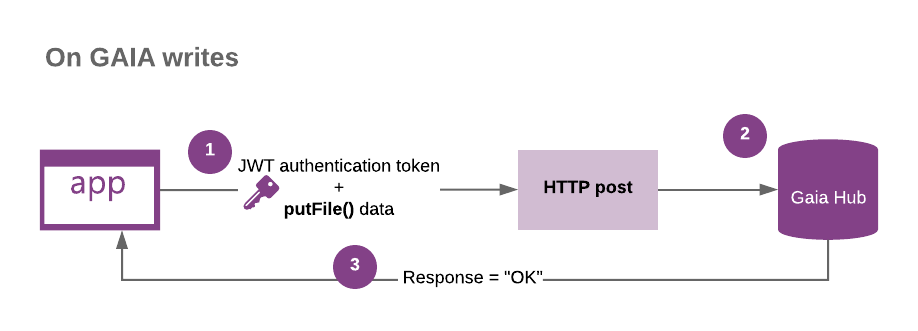
\includegraphics[width=\linewidth]{figures/gaia-writes}
			\caption{\label{fig:gaia-writes} The token ensures that a write is authorized\protect\footnotemark}
		\end{figure}
		\footnotetext{\url{https://docs.blockstack.org/storage/authentication.html}}
		
		Reading data from a user's Gaia hub involves a \textit{zonefile} lookup. This zonefile is a signed JSON object containing the URLs pointing to the user's Gaia data locker. Once verified that the zonefile is signed by user's key, a standard \texttt{HTTP} request is made to fetch the requested data.
		
		Figure~\ref{fig:gaia-overview} shows an overview of Gaia. Looking up data for a name works as follows:
		
		\begin{enumerate}
			\item Lookup the \textit{name} in the Virtualchain to get the (\textit{name, hash}) pair.
			\item Lookup the \textit{hash(name)} in Peer Network to get respective zonefile.
			\item Get the user's Gaia URL from the zonefile and lookup the URL to connect to storage backend.
			\item Fetch the requested data and verify the respective signature or hash.
		\end{enumerate}
		
		\begin{figure}[h]
			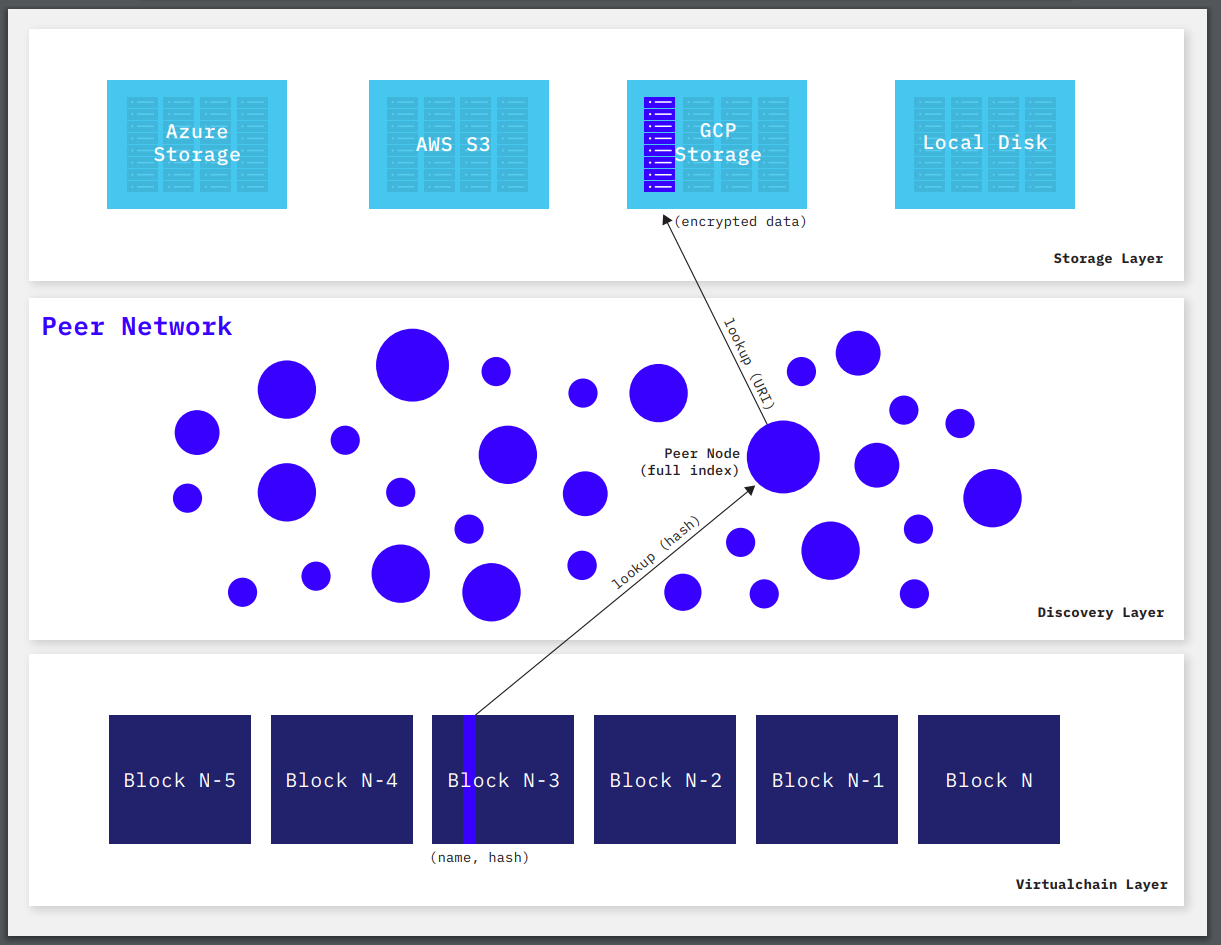
\includegraphics[width=\linewidth]{figures/gaia-overview}
			\caption{\label{fig:gaia-overview} Overview of Gaia and steps for looking up data.\protect\footnotemark}
		\end{figure}
		\footnotetext{\url{https://blockstack.org/whitepaper.pdf}}
		
	
\section{Identity}
	User identities are essential to using internet applications. In order to confirm their identity, users must provide some information. This information depends on the application's authentication process. If an application maintains a user database, it requires a username and a password and sometimes a second factor. If an application relies on a third-party, like Google\footnote{\url{https://developers.google.com/identity/}} or Facebook\footnote{\url{https://developers.facebook.com/docs/facebook-login/}} for identity management, it uses the OAuth 2.0 authentication\cite{hardt2012oauth} protocol, which identifies a user by generating an assertion from the identity service.
	
	Third party identity providers implementing the OAuth\footnote{\url{https://oauth.net/}} protocol often have their own version of implementation which leads to identity fragmentation across the web. OpenID\cite{recordon2006openid} is a decentralized identity protocol that allows users to create one identity which can be carried across multiple providers. However, the user still needs to trust one of the service providers with their identity information\cite{raval2016decentralized}.
	
	Another way of authenticating users with an application is by using digital certificates\cite{tycksen2001digital}. These certificates provide a proof of ownership of a public key. Authentication and management of public keys is facilitated using a Public Key Infrastructure (PKI)\cite{adams2003understanding} system. Currently, the most common approaches to PKIs are: Certificate Authorities (CAs) and PGP Web of Trust\cite{abdul1997pgp}. 
	
	A Certificate Authority (CA) acts a trusted third party responsible for management and distribution of digital certificates for a network of users\cite{fromknecht2014decentralized}. These trusted third parties introduces central control in a PKI system making them prone to single point of failure risk\cite{dooley2001designing}.
	
	In PGP Web of trust, authentication is entirely decentralized; users are able to designate others as trustworthy by signing their public keys. This process generates a digital certificate containing the user's public key and signatures from entities that have deemed him trustworthy. This system does benefit from its distributed nature as there is no central control. However, PGP does not offer identity retention. There is no guarantee of consistency and nothing prevents multiple users from creating public keys for the same identity\cite{fromknecht2014decentralized}.
	
	\subsection{Decentralized Public Key Infrastructure (DPKI)}
		\begin{figure}[h]
			\centering
			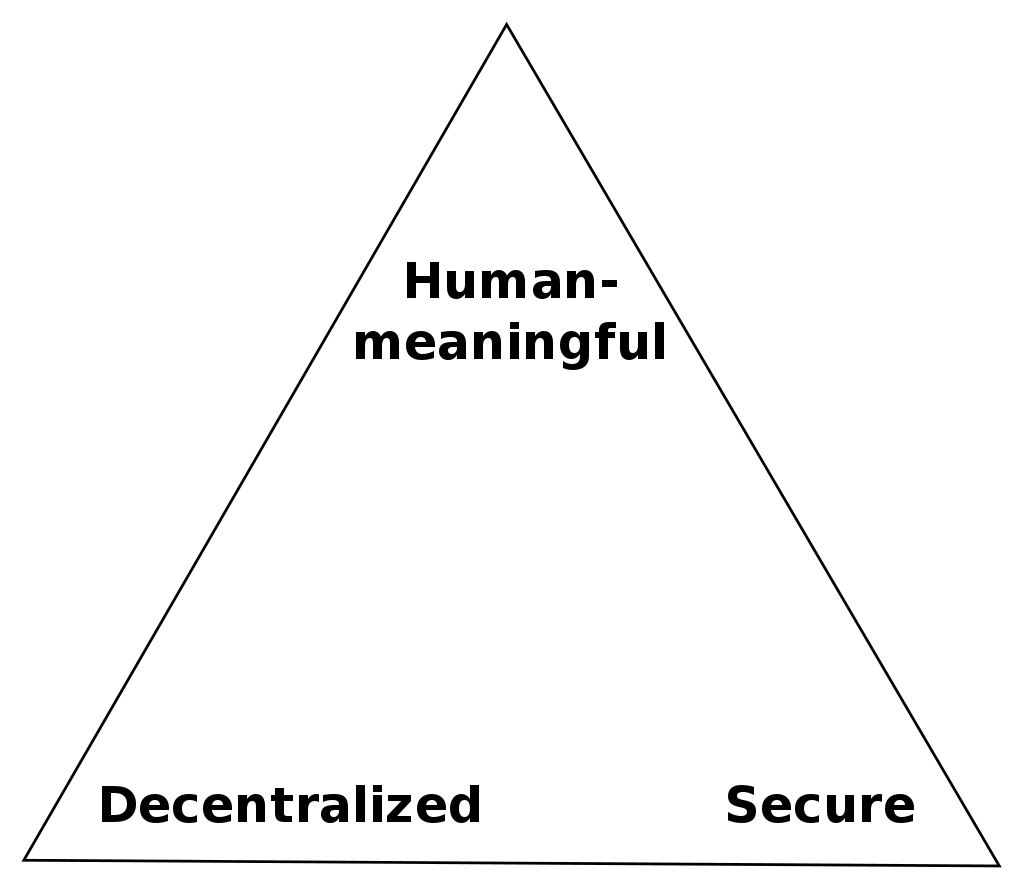
\includegraphics[width=200pt, height=150pt]{figures/zooko-triangle}
			\caption{\label{fig:zooko-triangle} Zooko's Triangle\protect\footnotemark}
		\end{figure}
		\footnotetext{\url{https://commons.wikimedia.org/wiki/File:Zooko\%27s_Triangle.svg}}
		
		The foundational precept of a DPKI is that \textit{identities belong to the entities they represent}. This requires designing a \textit{decentralized} infrastructure where every identity is controlled by its \textit{principal owner} and not by some trusted third party\cite{allen2015decentralized}.
		
		DPKI is essentially a system to gives unique names to participants in a network protocol. These names should have three desirable traits(Zooko's triangle) namely: \textit{Human-meaningful}, \textit{Decentralized} and \textit{Secure}. OpenID solved security and human-meaningfulness.
		
		Namecoin\footnote{\url{https://www.namecoin.org/}} was the first working solution that satisfied all three traits of Zooko's triangle by adding decentralization. It was the first fork of Bitcoin\cite{nakamoto2008bitcoin} protocol designed to act as a decentralized domain name server (DNS) for \textit{.bit} addresses. Namecoin's blockchain essentially could be used as an intermediary between a user and the service requesting user's identity\cite{raval2016decentralized}. It allowed a user to \textit{register} a name by creating a blockchain transaction. This transaction included the desired name which get embedded under the \textit{/id} namespace.
	
	\subsection{Decentralized Identifiers (DIDs)}
		A DID\footnote{\url{https://w3c-ccg.github.io/did-spec/}} is a new type of identifier that is globally unique, resolvable with high availability and cryptographically verifiable. DIDs typically contains cryptographic key pair which enables the controller of a DID to prove control over it.
		
		The concept of global unique decentralized identifiers is not new; Universally Unique Identifiers\footnote{\url{https://en.wikipedia.org/wiki/Universally_unique_identifier}}(UUIDs), also called Globally Unique Identifiers (GUIDs) were first such identifiers developed in 1980s and formally specified in RFC4122\footnote{\url{https://tools.ietf.org/html/rfc4122}}. Another class of identifiers knows as persistent identifiers was standardized as Uniform Resource Names (URNs) by RFC8141\footnote{\url{https://tools.ietf.org/html/rfc8141}}.
		
		However, UUIDs are not globally resolvable and URNs, if resolvable, require a central registry. Further, neither UUIDs or URNs have the ability to cryptographically verify ownership of the identifier. DIDs, on the other hand, fulfills all four requirements: persistence, global resolvability, cryptographically verifiability, and decentralization required for a self-sovereign identity\cite{smith2016identity}.
		
		\begin{figure}[h]
			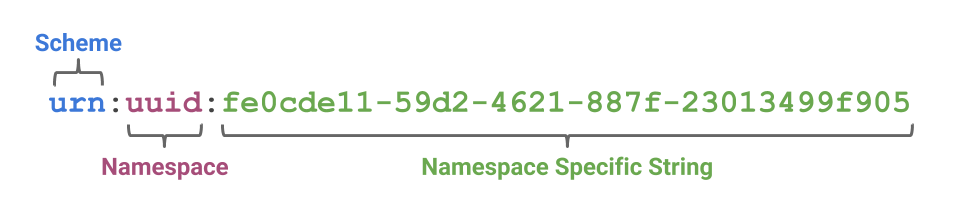
\includegraphics[width=\linewidth]{figures/urn-format}
			\caption{\label{fig:urn-format} The URN Specification}
		\end{figure}
	
		\begin{figure}[h]
			
\includegraphics[width=\linewidth]{figures/did-format}
			\caption{\label{fig:did-format} The DID Specification}
		\end{figure}
		
		The DID (Figure~\ref{fig:did-format}\footnote{\url{https://w3c-ccg.github.io/did-primer/did-primer-diagrams/did-format.png}}) specification follows the same pattern as the URN (Figure~\ref{fig:urn-format}\footnote{\url{https://w3c-ccg.github.io/did-primer/did-primer-diagrams/urn-format.png}}) specification. The key difference is that with DIDs, the namespace component identifies a \textit{DID method} which defines how DIDs work with a specific blockchain. The \textit{DID method} specifications must define the format and generation of the method-specific identifier. The DID methods can also be developed for identifiers registered in federated or centralized identity management systems, thus creating a interoperability bridge between the worlds of centralized, federated and decentralized identifiers.
	
	\subsection{Related Work}
		\subsubsection{Blockstack Authentication}\label{sec:blockstack-auth}
		Blockstack\footnote{\url{https://blockstack.org/}} is a decentralized computing network and app ecosystem that uses public-key cryptography and blockchain technology to provide its users with a DPKI system thereby making it possible to have a universal username that works across applications without the need for any passwords.
		
		\begin{figure}[h]
			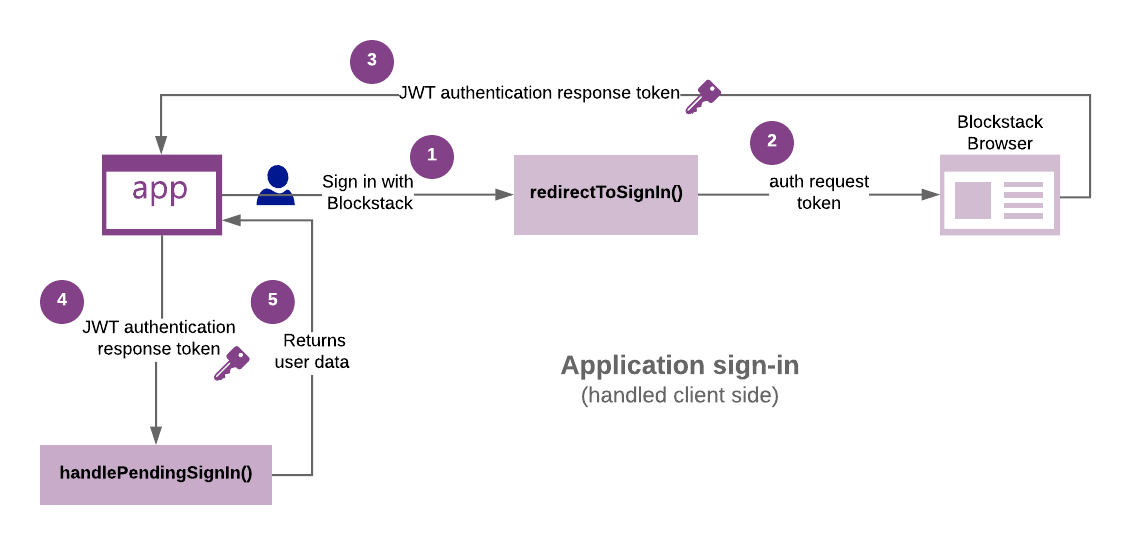
\includegraphics[width=\linewidth]{figures/app-sign-in}
			\caption{\label{fig:app-sign-in} Blockstack Authentication Flow\protect\footnotemark}
		\end{figure}
		\footnotetext{\url{https://docs.blockstack.org/storage/images/app-sign-in.png}}
		
		Blockstack Auth\footnote{\url{https://docs.blockstack.org/develop/overview_auth.html}} is a token-based authentication\footnote{\url{https://www.w3.org/2001/sw/Europe/events/foaf-galway/papers/fp/token_based_authentication/}} system. When a user signs into an application, an \texttt{authRequest} token is sent to the Blockstack Browser. Once the sign-in is approved, the Blockstack Browser responds with an \texttt{authResponse} token. This response provides the application with enough information to generate and store authentication data. Since all usernames are registered on the blockchain, every application have an up-to-date view of all usernames and corresponding public keys. This eliminates the need for a server-side identity provider.
	
		Figure~\ref{fig:app-sign-in} visualizes the authentication flow for an application using Blockstack Auth. When a user chooses to \textbf{Sign in with Blockstack}, it calls the \texttt{redirectToSignIn()} method which sends an \texttt{authRequest} token to the Blockstack Browser\footnote{\url{https://github.com/blockstack/blockstack-browser}}. Upon receiving the request, the Blockstack Browser presents the user with a choice of IDs to use to sign in, as well as a list of permissions the application needs. Upon selecting an ID, the Blockstack Browser redirects back to the application with a \texttt{authResponse} token containing three pieces of information\footnote{\url{https://blockstack.org/whitepaper.pdf}}:
		\begin{itemize}
			\item The user's username (or the hash of the public key if no username is set).
			\item An \textit{application-specific} private key for encrypting and signing user's data. This key is deterministically  generated from the user's master private key, the ID used to sign in, and the application's HTTP Origin.
			\item The URLs to the user private data locker (Gaia Hub\footnote{\url{https://github.com/blockstack/gaia/tree/master/hub}}).
		\end{itemize}
		
		Above pieces of information instructs the application on how to find and store a user's data on their behalf.
	
\section{Value}
	Value help us to quantify quantities of an asset in order to make them measurable\footnote{\url{https://medium.com/swlh/what-is-the-internet-of-values-3f14b5d35a90}}. It can mean money, intellectual property or securities. In traditional internet applications trust is required in a third-party (a bank or a financial institution) when transferring value between two entities. While this system works well enough for most transactions, it still suffers from the inherent weaknesses of the trust based model\cite{nakamoto2008bitcoin}.
	
	\begin{figure}[h]
		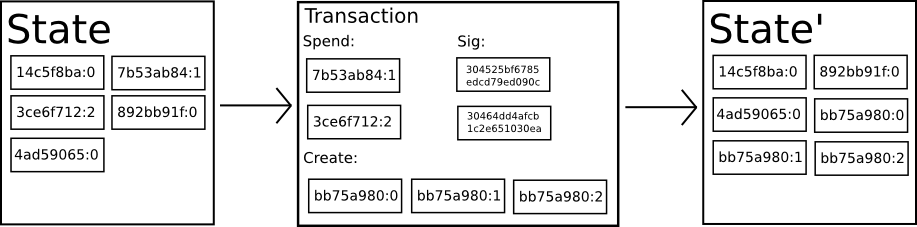
\includegraphics[width=\linewidth]{figures/state-transition}
		\caption{\label{fig:state-transition} Bitcoin as a state transition system\protect\footnotemark}
	\end{figure}
	\footnotetext{\url{https://raw.githubusercontent.com/ethereumbuilders/GitBook/master/en/vitalik-diagrams/statetransition.png}}
	
	Bitcoin\cite{nakamoto2008bitcoin} was the first peer-to-peer electronic payment system that's based on cryptographic proof instead of trust, allowing any two entities to transfer value over the internet without the need for any trusted third-party. A transaction in the Bitcoin network involves digitally signing a hash of the previous transaction and the public key of the recipient and adding these to the end of the transaction. Multiple transactions are combined to form a block and each block is linked with the previous block by it's hash and a \textit{nonce} generated by a proof-of-work\cite{back2002hashcash} algorithm. This chain of blocks forms a distributed data structure called the \textit{blockchain}. It can be thought of as a state transition system, where a \textit{state} consists of the ownership status of all existing bitcoins and a \textit{state transition function} that takes a state and a transaction and outputs a new state\cite{buterin2014ethereum}.
	
	\begin{figure}[h]
		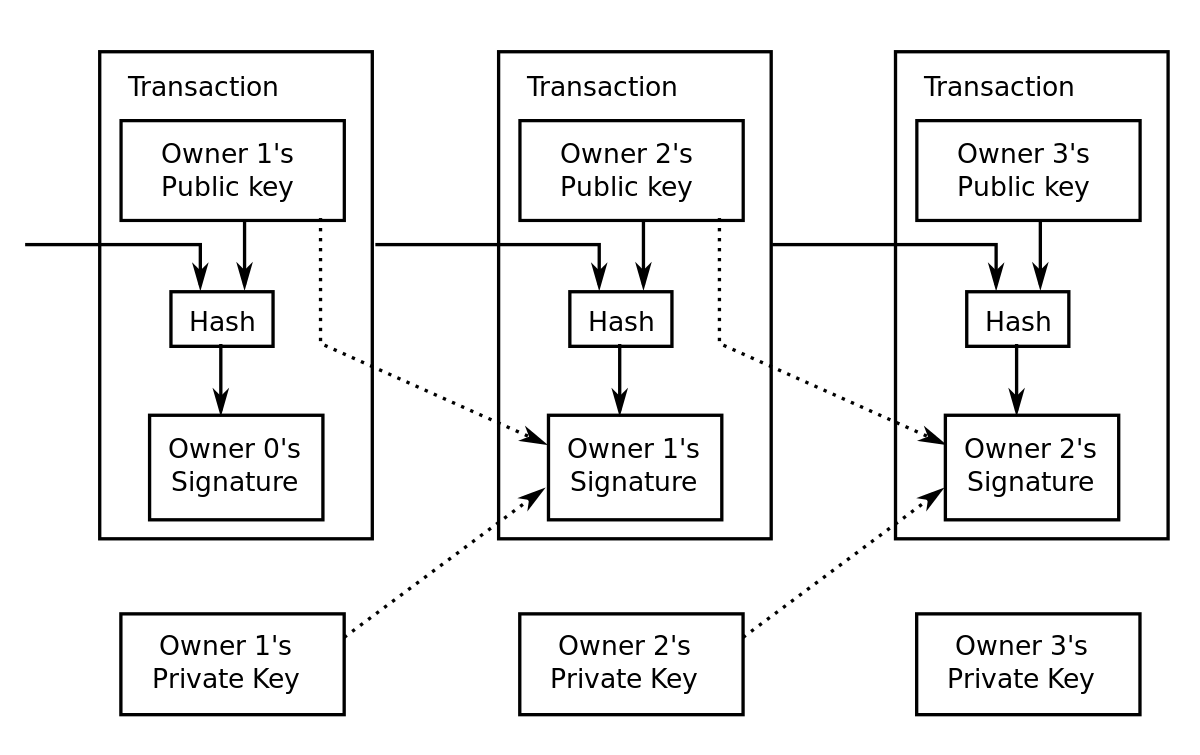
\includegraphics[width=\linewidth]{figures/bitcoin-transactions}
		\caption{\label{fig:bitcoin-transactions} Transactions in the Bitcoin Network\protect\footnotemark}
	\end{figure}
	\footnotetext{\url{https://cdn-images-1.medium.com/max/1200/1*d9AIfrD_DOLtXfKVnadN6w.png}}
	
	Blockchain, the underlying technology of Bitcoin can also be applied to build systems which can represent assets in the physical world. For example, \textit{Secure property titles with owner authority\footnote{\url{https://nakamotoinstitute.org/secure-property-titles/}}}, a document written by Nick Szabo\footnote{\url{https://en.wikipedia.org/wiki/Nick_Szabo}} describes how a blockchain-based system can be used to build a land registry. Ethereum\cite{buterin2014ethereum}, an alternative protocol with a built-in Turing-complete programming language enables such systems by allowing anyone to write \textit{smart contracts}\cite{szabo1997formalizing} where they can create their own arbitrary rules of ownership\footnote{\url{https://github.com/ethereum/wiki/wiki/White-Paper}}.
	
	Ethereum also enables the creation of \textit{tokens} which allows us to represent something specific in an application, for example, economic value, a dividend, a stake or even a voting right\footnote{\url{https://education.district0x.io/general-topics/understanding-ethereum/the-role-of-tokens/}}. The two most common tokens standards in the Ethereum ecosystem are \textit{ERC-20}\footnote{\url{https://github.com/ethereum/EIPs/blob/master/EIPS/eip-20.md}}: A class of identical tokens, and \textit{ERC-721}\footnote{\url{https://github.com/ethereum/EIPs/blob/master/EIPS/eip-721.md}}: A class of unique tokens. These token standards can be used to tokenize ownership of any arbitrary data or even real world assets thereby enabling an \textit{Internet of Value}\footnote{\url{https://hackernoon.com/a-vision-of-the-internet-of-value-ad187abf5826}}.
	
\section{Computing}
	Any web application needs computing resources to work. Traditional internet relied on a \textit{client-server} model where server is usually a more powerful, better connected machine and thus provided most of the computing resources. This, however, also made server as a single bottleneck for performance and reliability\cite{crowcroft2003peer}. As internet connectivity improved and web applications became more complex, the demand for computing resources increased.
	
	Virtualization\footnote{\url{http://www.kernelthread.com/publications/virtualization/}}, a concept pioneered by the VM\cite{creasy1981origin} operating system led to the emergence of \textit{cloud computing}. Cloud computing satisfied the growing demand of web applications by providing an on-demand delivery of computing resources over the internet. This greatly defined the current internet architecture where applications relies on cloud services providers who provides computing resources based on different service models (Figure~\ref{fig:service-models}).
	
	\begin{figure}[h]
		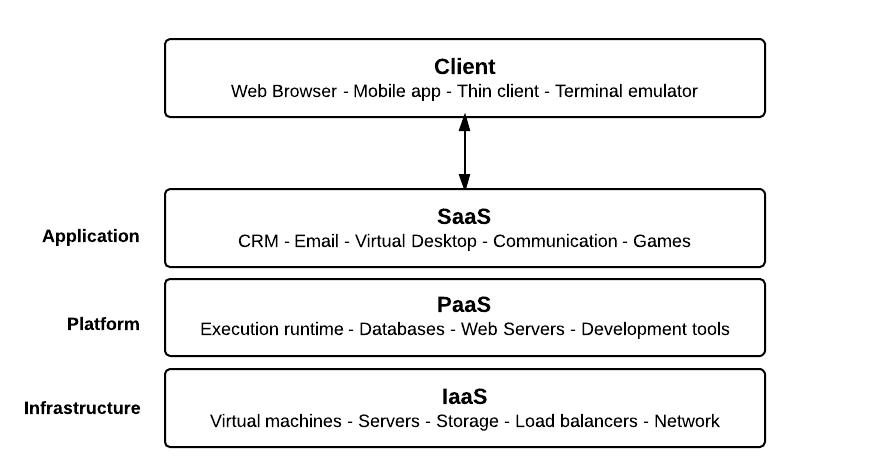
\includegraphics[width=\linewidth]{figures/service-models}
		\caption{\label{fig:service-models} Cloud computing service models\protect\footnotemark}
	\end{figure}
	\footnotetext{\url{https://static.bluepiit.com/blog/wp-content/uploads/sites/2/2015/12/types-of-cloud-computing-models.png}}
	
	Cloud computing, however, poses privacy concerns as it requires entrusting data to information systems managed by third-party cloud service providers who has access to all of user's data at any time and could accidentally or deliberately use it for unauthorized purposes\cite{ryan2011cloud}. Because data from multiple entities can be stored on a large cloud servers, it poses security concerns as well. Hackers can theoretically gain control of huge amounts of data through a single attack - a process called \textit{hyperjacking}\footnote{\url{https://www.securityweek.com/deep-dive-hyperjacking}}.
	
	Blockchain can be used to create a decentralized global market where infrastructure providers,  application owners and individual users can come together to trade their unused computing resources. This will also allow us to harness the computing resources of millions of personal computers and workstations connected to the public internet which have hundreds of compute cycles going unused every second\cite{crowcroft2003peer}. Coupled with end-to-end encryption, this network of connected computers can overcome the security and privacy concerns posed by Cloud computing.
	
	\subsection{Related Work}
		\subsubsection{Golem Network}
		Golem\footnote{\url{https://golem.network/crowdfunding/Golemwhitepaper.pdf}} aims to create a decentralized supercomputer by creating a global market for computing power. It connects computers in a peer-to-peer network, enabling every participant to share their unused resources. It uses the Ethereum blockchain for accounting, which enables direct payments between providers, application owners and individual users. Finally, it employs an \textit{Application Registry} which is an Ethereum smart contract, to which anyone can publish their application.
		
		\begin{figure}[h]
			\centering
			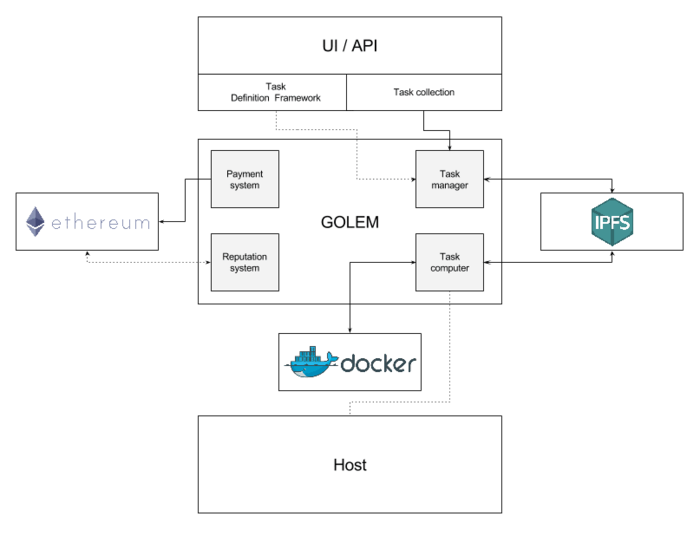
\includegraphics[width=\linewidth]{figures/golem-network}
			\caption{\label{fig:golem-network} Overview of Golem Network Architecture\protect\footnotemark}
		\end{figure}
		\footnotetext{Adapted from \url{https://en.bitcoinwiki.org/wiki/Golem_Worldwide_Supercomputer}}
	
\section{Bandwidth}
	ISPs act as gateways between end users and the internet (Figure~\ref{fig:internet-backbone}). They solve the "last mile" problem by connecting users to the high-speed internet and acting as a central hub for communication. However, these central gateways are also central points of failure. Governments can shut them down or ask them to blacklist certain IPs\cite{raval2016decentralized}.
	
	\begin{figure}[h]
		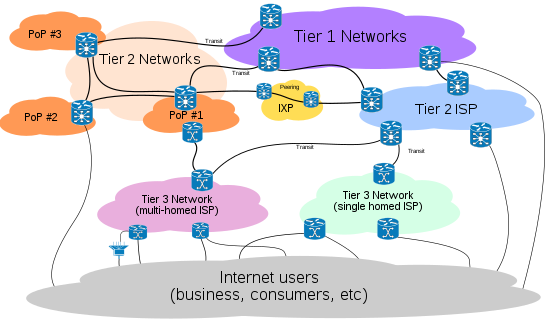
\includegraphics[width=\linewidth]{figures/internet-backbone}
		\caption{\label{fig:internet-backbone} The Internet\protect\footnotemark}
	\end{figure}
	\footnotetext{\url{https://commons.wikimedia.org/wiki/File:Internet\_Connectivity\_Distribution\_\%26_Core.svg}}
	
	Mesh networks are the decentralized version of standards internet where users don't need to go through a central gateway. In a mesh network, nodes connect to as many adjacent nodes for efficient routing of data. However, a decentralized consensus system is required to incentivize all participants to share their bandwidth. Blockchain can used to serve as an incentive layer effectively creating a decentralized marketplace for bandwidth. Mark Nadal and Dr. Amber Cazzell describes one such protocol in their paper \textit{A Trustless Decentralized Bandwidth Incentive}\footnote{\url{https://web.stanford.edu/~nadal/A-Decentralized-Data-Synchronization-Protocol.pdf}}.
	
	\subsection{Related Work}
		\subsubsection{NOIA Network}
		NOIA\footnote{\url{https://noia.network/}} network is a Distributed peer-to-peer content delivery network, governed by the blockchain where nodes are incentivized for providing storage and unused bandwidth to the network.
		
		\begin{figure}[h]
			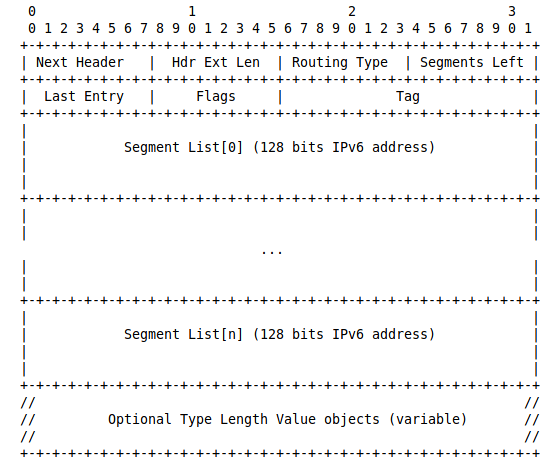
\includegraphics[width=\linewidth]{figures/ipv6-segment-header}
			\caption{\label{fig:segment-header} IPv6 Segment Routing Header\protect\footnotemark}
		\end{figure}
		\footnotetext{\url{https://docs.noia.network/noia/segment-routing--srv6-}}
		
		NOIA enables a \textit{programmable internet}\footnote{\url{https://docs.noia.network/noia/programmable-internet}} by leveraging IPv6 and Segment Routing (SR). IPv6 increases the address size from 32 bits to 128 bits. This increase in packet size allows NOIA to encode custom information in packet headers thus providing an identification system for nodes connected to the network. These \textit{custom headers} (Figure~\ref{fig:segment-header}) enables SR by leveraging the source routing paradigm. SR is then used to create a Software Defined Network (SDN) where nodes are identified by their segment identifiers (SIDs). SIDs are registered on the NOIA Ledger to create a network topology of SR enabled access points. A Decentralized Internet Transit Exchange (DITEX) is used for trading of access points as a Transit.
		
		\subsubsection{Althea Network}
		Althea\footnote{\url{https://althea.net/}} Network aims to solve the "last mile" problem by connecting a source of internet connectivity to the end users using a mesh network topology where packets are forwarded using the Babel routing protocol\cite{chroboczek2011babel}. It creates a decentralized ISP where routers pay each other for bandwidth with cryptocurrencies. Governance in Althea network is done using a \textit{proof-of-stake} blockchain built using the Cosmos\footnote{\url{https://cosmos.network/}} protocol.
		
		\begin{figure}[h]
			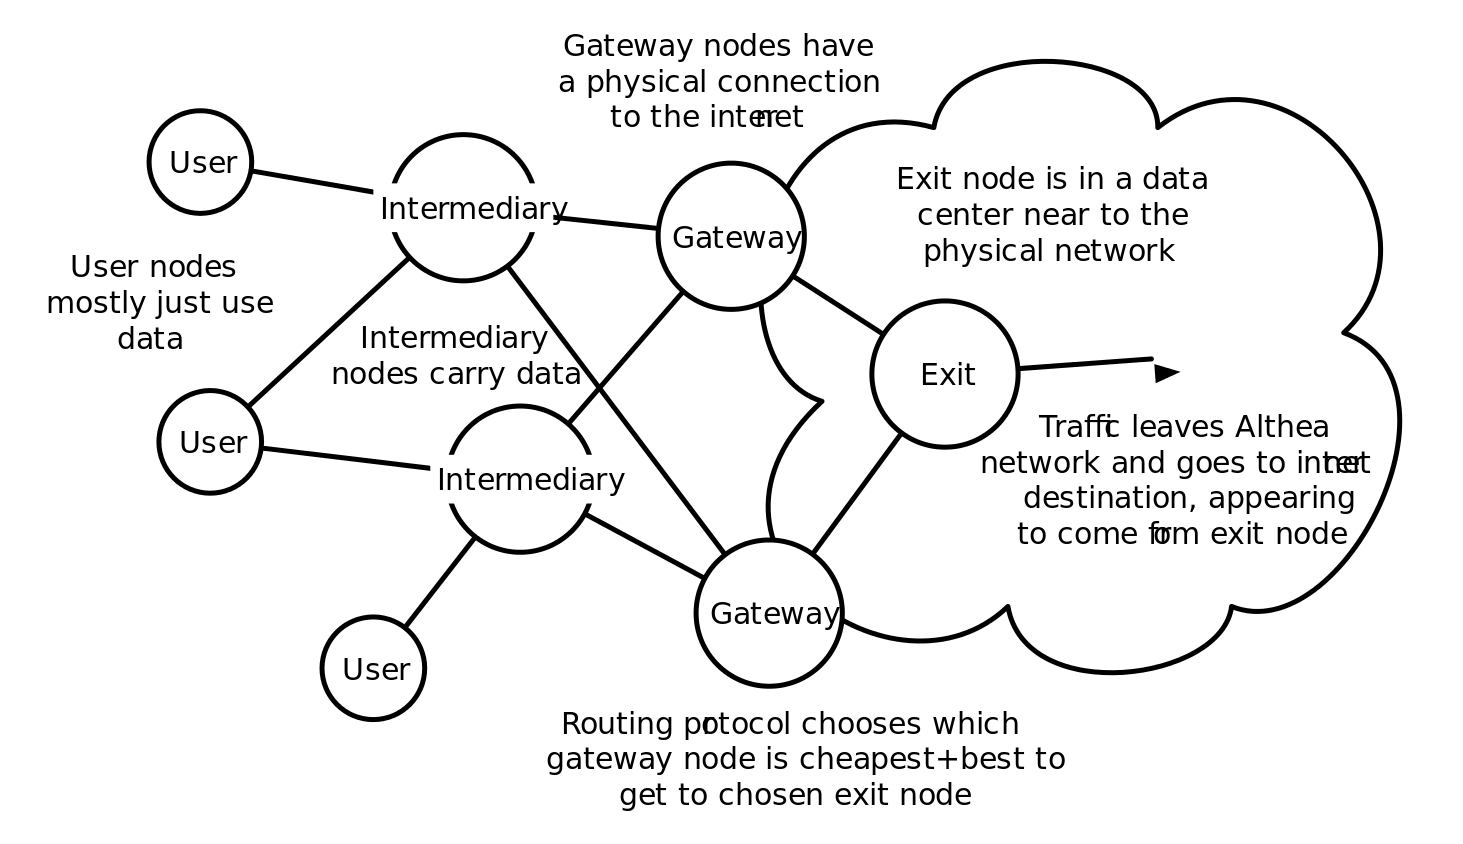
\includegraphics[width=\linewidth]{figures/althea-network}
			\caption{\label{fig:althea-network} The Althea Network\protect\footnotemark}
		\end{figure}
		\footnotetext{Adapted from: \url{https://althea.net/whitepaper}}
	
\section{Application Design}
	Designing any web application requires understanding of the underlying architecture. This section combines all the application concepts to visualize the underlying architecture which enables decentralized applications with data ownership.
	
	\subsection{Decentralized Application Architecture}
	Self-sovereign identity is one of the most important element in decentralized applications with data ownership.  The DIDs\footnote{\url{https://w3c-ccg.github.io/did-spec/}} specifications enables the creation of a DPKI system on top of any blockchain. A user can create a \textit{decentralized identity} by registering their public key with a desired username by creating a blockchain transaction.
	
	\begin{figure}[h]
		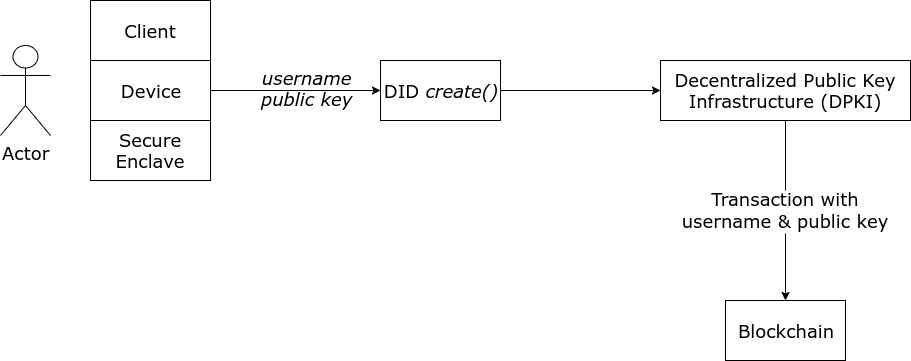
\includegraphics[width=\linewidth]{figures/did-create}
		\caption{\label{fig:did-create} Creating a Decentralized Identity}
	\end{figure}
	
	A decentralized identity anchored on a blockchain serves two purposes. First, it gives us a cryptographic keypair which can be used by an application for encryption/decryption of data. Second, it serves as a digital wallet for secure exchange of value across the Internet using cryptocurrencies.
	
	Decentralized applications follow a \textit{serverless} architecture where backend services such as database, storage and authentication are provided as APIs that enable client applications to connect directly to these services. The frontend components such as business logic and application code are deployed inside a hosting environment such that the servers that run the code is completely abstracted.
	
	\begin{figure}[h]
		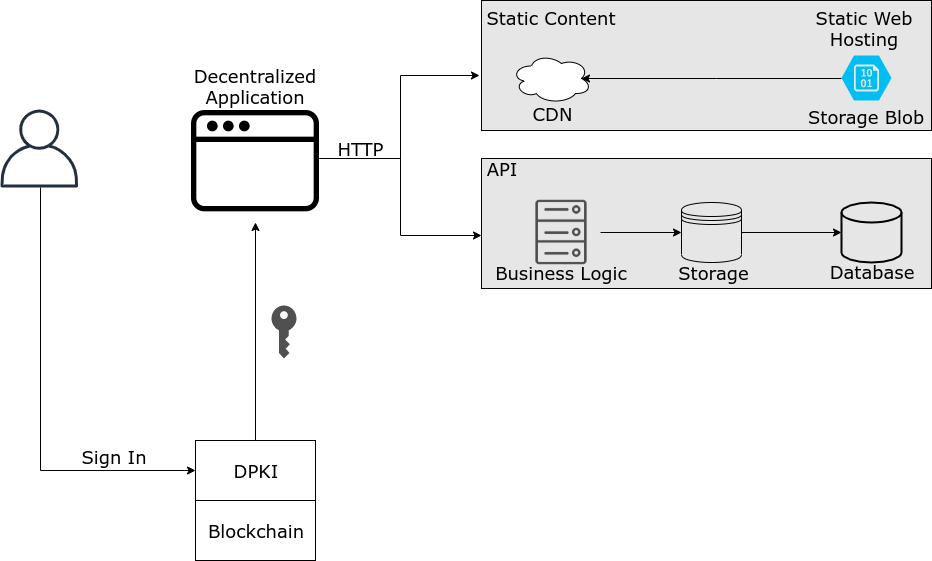
\includegraphics[width=\linewidth]{figures/dapp-architecture}
		\caption{\label{fig:dapp-architecture} Decentralized Application Architecture}
	\end{figure}

	Figure~\ref{fig:dapp-architecture} visualizes the architecture of a decentralized web application. Authentication is handled using a DPKI system. The application connects to various services like storage and database using APIs. The client application encrypts all private data using user's public key before sending it to a decentralized storage network. A database service can be used for easy indexing of data.
	
\section{Summary}
	This chapter outlined the different concepts of a web application and showed how Blockchain enables decentralization for each of the concepts. The key concept which allows us to build decentralized applications with data ownership is \textit{Decentralized Identity}. It enables a Web where we don't have to use username/passwords anymore and where our data have cryptographic security.